\subsection*{Phần 1: Trường bên trong lớp trụ}
\begin{wrapfigure}[4]{r}{6cm}
  \centering
  \vspace{-12mm}
  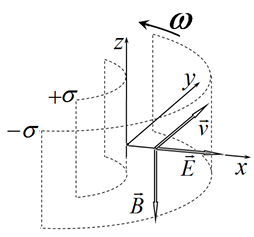
\includegraphics[width=0.25\textwidth]{Figures/P2/Fig 2.1S.png}
\end{wrapfigure}

\noindent\textbf{1.} Hướng của các vector được chỉ ra trên hình vẽ:
\begin{itemize}
  \item Vector $\vec{E}$ hướng dọc theo trục $x$;
  \item Vector $\vec{B}$ hướng ngược chiều trục $z$;
  \item Vector $\vec{v}$ hướng dọc theo trục $y$.
\end{itemize}

\noindent\textbf{2.} Khi quay một hình trụ được tích điện đều, ta có thể xem nó như một ống dây solenoid có mật độ vòng $n$ mang dòng điện có cường độ $I$ với:
\begin{equation*}
  nl=\sigma v=\sigma\omega R
\end{equation*}
do đó, cảm ứng từ bên trong lớp trụ là:
\begin{equation*}
  B=\mu_{0}\sigma\omega R
\end{equation*}

\noindent\textbf{3.} Hướng của các lực được chỉ ra trên hình vẽ:
\begin{figure}[h]
  \centering
  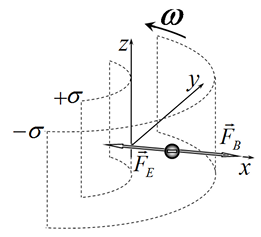
\includegraphics[width=0.23\textwidth]{Figures/P2/Fig 2.2S.png}
\end{figure}

\noindent\textbf{4.} Độ lớn của lực điện:
\begin{equation*}
  F_{E}=eE=e\frac{\sigma}{\varepsilon_{0}}
\end{equation*}
vì các vector vận tốc và cảm ứng từ vuông góc với nhau, độ lớn của lực từ là:
\begin{equation*}
  F_{B}=evB=e(\omega R)(\mu_{0}\sigma\omega R)=e\mu_{0}(\omega^{2}R^{2})\sigma
\end{equation*}

\subsection*{Phần 2: Điện tích và dòng điện}
\begin{wrapfigure}[8]{r}{6cm}
  \centering
  \vspace{-4mm}
  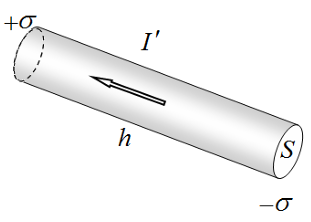
\includegraphics[width=0.3\textwidth]{Figures/P2/Fig 2.3S.png}
\end{wrapfigure}


\noindent\textbf{1.} Rõ ràng, sự thay đổi điện tích trên bề mặt lớp xảy ra nhờ dòng điện chạy ngang qua lớp được chọn. Xét một hình trụ nhỏ nằm giữa hai mặt bên của lớp trụ có trục đối xứng vuông góc với với trục của lớp trụ. Gọi diện tích mặt cắt của vỏ trụ này là $S$, chiều dài của nó bằng độ dày của lớp và bằng $h$. SỰ thay đổi điện tích trên mặt trụ bằng cường độ dòng điện $I'$ chạy qua nó:
\begin{equation*}
  \frac{\Delta(\sigma S)}{\Delta t}=I'
\end{equation*}
để tính cường độ dòng điện, ta có thể sử dụng định luật Ohm. Trong trường hợp này, hiệu điện thế hiệu dụng là:
\begin{equation*}
  U_{\text{eff}}=\frac{F_{E}-F_{B}}{e}h
\end{equation*}
điện trở là:
\begin{equation*}
  R=\rho\frac{h}{S}
\end{equation*}
suy ra:
\begin{equation*}
  \frac{\Delta(\sigma S)}{\Delta t}=\frac{U_{\text{eff}}}{R}=\frac{\sigma}{\rho \varepsilon_{0}}\left[\varepsilon_{0}\mu_{0}(\omega R)^{2}-1\right]S
\end{equation*}
như vậy:
\begin{equation*}
  \frac{\Delta\sigma}{\Delta t}=\frac{\sigma}{\rho \varepsilon_{0}}\left[\varepsilon_{0}\mu_{0}(\omega R)^{2}-1\right]
\end{equation*}

\noindent\textbf{2.} Cảm ứng từ sẽ tăng nếu tốc độ thay đổi điện tích là dương, tức là khi:
\begin{equation*}
  \varepsilon_{0}\mu_{0}(\omega R)^{2}-1>0\implies V^{*}=\omega^{*}R=\frac{1}{\sqrt{\varepsilon_{0}\mu_{0}}}=c\approx 3.10^{8}\SI{}{\metre\second^{-1}}
\end{equation*}

\noindent\textbf{3.} Ta có:
\begin{equation*}
  \omega^{*}R=c\implies \omega^{*}=\frac{c}{R}
\end{equation*}
thời gian một ngày trên Trái Đất bằng chu kì quay của Trái Đất quanh trục:
\begin{equation*}
  T=\frac{2\pi}{\omega^{*}}=\frac{2\pi R}{c}\approx 0,073\SI{}{\second}
\end{equation*}

\noindent\textbf{4.} Tốc độ của lớp được chọn:
\begin{equation*}
  V=\frac{2\pi R}{T}\approx 5,2.10^{2}\SI{}{\metre\second^{-1}}
\end{equation*}
giá trị này rất nhỏ so với tốc độ ánh sáng. Tỷ lệ giữa lực từ và lực điện tác dụng lên electron là:
\begin{equation*}
  \varepsilon_{0}\mu_{0}(\omega R)^{2}=\left(\frac{V}{c}\right)^{2}\approx 7,2.10^{-13}
\end{equation*}
giá trị này là rất nhỏ so nên ta có thể bỏ qua, khi đó:
\begin{equation*}
  \frac{\Delta\sigma}{\Delta t}=-\frac{\sigma}{\rho\varepsilon_{0}}
\end{equation*}
thời gian đặc trưng:
\begin{equation*}
  \tau=\frac{\sigma_{0}}{\lvert \dfrac{\Delta\sigma}{\Delta t}\rvert _{0}}=\rho\varepsilon_{0}\approx1,2.10^{-17}\SI{}{\second}
\end{equation*}

\subsection*{Phần 3: Khối lượng của electron có cứu mô hình này không?}
\noindent\textbf{1.} Khi tính đến khối lượng của electron, ta phải xét đến gia tốc hướng tâm của nó:
\begin{equation*}
  eE=m_{e}\omega^{2}R
\end{equation*}
từ đó suy ra mật độ điện tích tính là:
\begin{equation*}
  \overline{\sigma}=\frac{m_{e}}{e}\varepsilon_{0}\omega^{2}R
\end{equation*}

\noindent\textbf{2.} Cảm ứng từ do các điện tích này tạo ra được xác định bởi:
\begin{equation*}
  B=\mu_{0}\overline{\sigma}\omega R=\frac{m_{e}}{e}\varepsilon_{0}\mu_{0}\frac{(\omega R)^{3}}{R}\approx2,8.10^{-28}\SI{}{\tesla}
\end{equation*}
giá trị này nhỏ hơn cảm ứng từ của Trái Đất 23 bậc.

\noindent\textbf{3.} Mô hình ta đã xét không thể mô tả được sự hình thành từ trường của Trái Đất.
